\documentclass{../../slides-style}

\slidetitle{Примитивы синхронизации}{14.09.2022}

\begin{document}

    \begin{frame}[plain]
        \titlepage
    \end{frame}

    \section{Синхронизация}

    \begin{frame}
        \frametitle{Примитивы синхронизации}
        \begin{itemize}
            \item Лучше необходимости синхронизации вообще избегать
            \item Бывают:
            \begin{itemize}
                \item User-mode --- атомарные операции, реализующиеся на процессоре и не требующие участия планировщика
                \item Kernel-mode --- примитивы, управляющие тем, как поток обрабатывается планировщиком
                \begin{itemize}
                    \item Более тяжеловесные и медленные (до 1000 раз по сравнению с ``без синхронизации вообще'')
                    \item Позволяют синхронизировать даже разные процессы
                \end{itemize}
            \end{itemize}
        \end{itemize}
    \end{frame}

    \section{Атомарные операции}

    \begin{frame}
        \frametitle{Атомарные операции}
        \begin{itemize}
            \item Чтения и записи следующих типов всегда атомарны: Boolean, Char, (S)Byte, (U)Int16, (U)Int32, (U)IntPtr, Single, ссылочные типы
            \item Для других типов (например, Int64) операции чтения и записи могут быть прерваны посередине!
        \end{itemize}
    \end{frame}

    \section{Volatile}

    \begin{frame}
        \frametitle{Volatile и модель памяти}
            \begin{center}
                \begin{tabu} {X[1 c p] X[1 c p]}
                    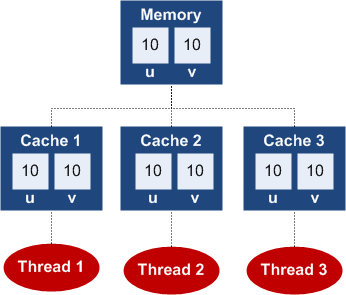
\includegraphics[width=0.25\textwidth]{volatile1.png} & 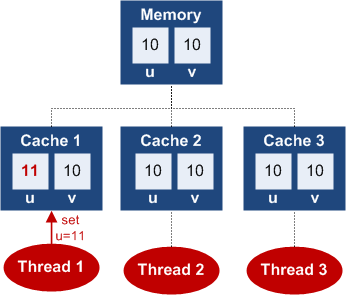
\includegraphics[width=0.25\textwidth]{volatile2.png} \\
                    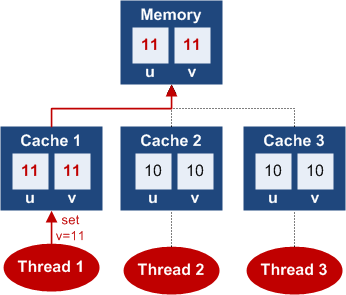
\includegraphics[width=0.25\textwidth]{volatile3.png} & 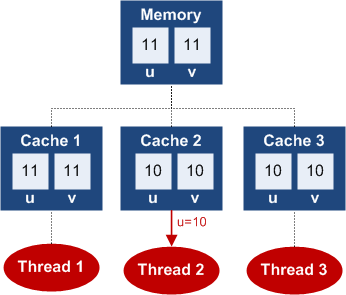
\includegraphics[width=0.25\textwidth]{volatile4.png} \\
                \end{tabu}
                \attribution{\url{https://igoro.com/archive/volatile-keyword-in-c-memory-model-explained/}}
            \end{center}
    \end{frame}

    \begin{frame}
        \frametitle{Volatile в .NET}
        \begin{itemize}
            \item \mintinline{csharp}|Volatile|
            \begin{itemize}
                \item \mintinline{csharp}|Volatile.Write|
                \item \mintinline{csharp}|Volatile.Read|
                \item Связано с понятием Memory Fence, требует синхронизации ядер
                \item Есть ключевое слово \mintinline{csharp}|volatile|: \mintinline{csharp}|private volatile int flag = 0;|
                \item \mintinline{csharp}|Volatile.Write| должен быть последней операцией записи, \mintinline{csharp}|Volatile.Read| --- первой операцией чтения
            \end{itemize}
        \end{itemize}
    \end{frame}

    \begin{frame}[fragile]
        \frametitle{Пример}
        \begin{minted}{csharp}
private int flag = 0;
private int value = 0;

public void Thread1() {
    value = 5;
    Volatile.Write(ref flag, 1);
}

public void Thread2() {
    if (Volatile.Read(ref flag) == 1)
        Console.WriteLine(value);
}
        \end{minted}
    \end{frame}

    \begin{frame}[fragile]
        \frametitle{Ещё один способ прострелить себе ногу}
        \begin{minted}{csharp}
static void Main(string[] args)
{
    var stop = false;
    var thread = new Thread(() => {
        stop = true;
    });

    thread.Start();

    while (!stop);

    thread.Join();

    Console.WriteLine("Done.");
}
        \end{minted}
    \end{frame}

    \section{Interlocked}

    \begin{frame}[fragile]
        \frametitle{Interlocked}
        \begin{small}
            \begin{columns}
                \begin{column}{0.4\textwidth}
                    \begin{minted}{csharp}
public int  result;

public void ThreadA()
{
    for (int i = 1; i <= 1000; i++) 
    {
        result++;
    }
}

public void ThreadB()
{
    for (int i = 1; i <= 1000; i++) 
    {
        result++; 
    }
}
                    \end{minted}
                \end{column}
                \begin{column}{0.05\textwidth}
                    \rule{0.1mm}{0.8\textheight}
                \end{column}
                \begin{column}{0.5\textwidth}
                    \begin{minted}{csharp}
public int  result;

public void ThreadA()
{
    for (int i = 1; i <= 1000; i++) 
    {
        Interlocked.Increment(ref result);
    }
}

public void ThreadB()
{
    for (int i = 1; i <= 1000; i++) 
    {
        Interlocked.Increment(ref result); 
    }
}
                    \end{minted}
                \end{column}
            \end{columns}
        \end{small}
    \end{frame}

    \section{Активное ожидание}

    \begin{frame}
        \frametitle{Критические области}
        \begin{center}
            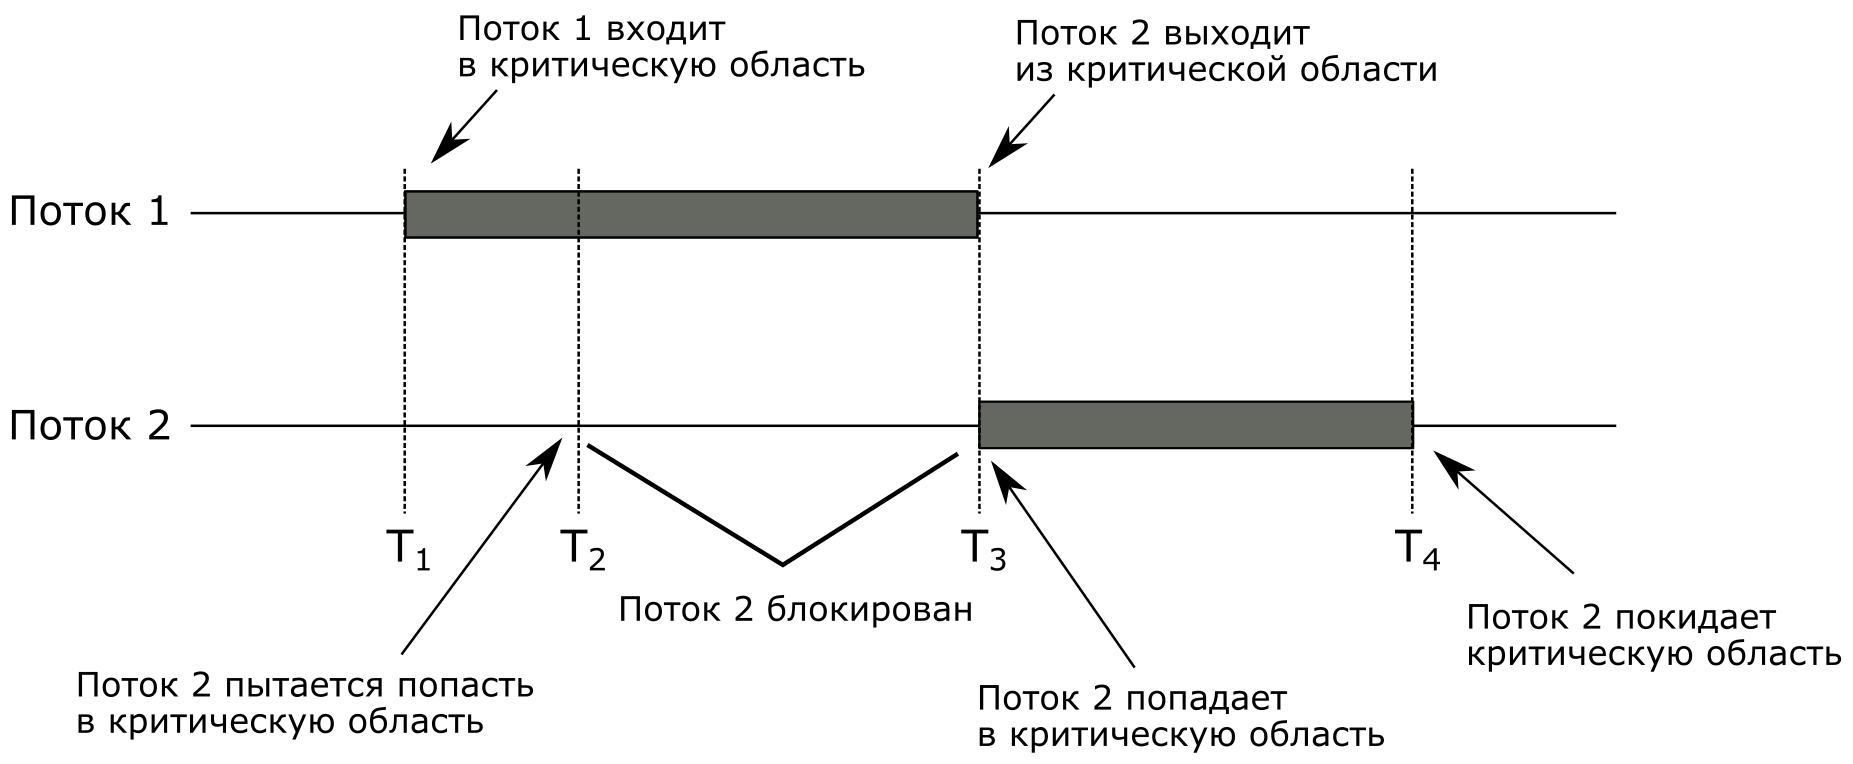
\includegraphics[width=0.9\textwidth]{criticalSections.png}
        \end{center}
    \end{frame}

    \begin{frame}[fragile]
        \frametitle{Активное ожидание}
        \begin{scriptsize}
            \begin{minted}{csharp}
private int turn = 0;

void Task1()
{
    while (true)
    {
        while (turn != 0);
        CriticalSection();
        turn = 1;
        NonCriticalSection();
    }
}

void Task2()
{
    while (true)
    {
        while (turn != 1) ;
        CriticalSection();
        turn = 0;
        NonCriticalSection();
    }
}
            \end{minted}
        \end{scriptsize}
    \end{frame}

    \begin{frame}
        \frametitle{Активное ожидание, обсуждение}
        \begin{itemize}
            \item Не требует поддержки ОС
            \begin{itemize}
                \item Поэтому переключение может быть очень быстрым
            \end{itemize}
            \item Ждущий поток полностью занимает ядро
            \begin{itemize}
                \item Греет процессор и очень быстро сажает аккумулятор
            \end{itemize}
            \item Потоки работают строго по очереди
            \begin{itemize}
                \item Это можно побороть, есть алгоритм Петерсона
            \end{itemize}
        \end{itemize}
    \end{frame}

    \begin{frame}[fragile]
        \frametitle{Проблема производителя и потребителя}
        \framesubtitle{Producer-consumer problem}
        \begin{footnotesize}
            \begin{minted}{csharp}
private Queue<int> buffer = new Queue<int>();
            \end{minted}
            \begin{columns}
                \begin{column}{0.5\textwidth}
                    \begin{minted}{csharp}
private void Producer() {
    while (true) {
        var item = ProduceItem();
        if (buffer.Count == 100)
            Sleep();
        buffer.Enqueue(item);
        if (buffer.Count == 1)
            WakeUp(Consumer);
    }
}
                    \end{minted}
                \end{column}
                \begin{column}{0.5\textwidth}
                    \begin{minted}{csharp}
private void Consumer() {
    while (true) {
        if (buffer.Count == 0)
            Sleep();
        var item = buffer.Dequeue();
        if (buffer.Count == 100 - 1)
            WakeUp(Producer);
        ConsumeItem(item);
    }
}
                    \end{minted}
                \end{column}
            \end{columns}
        \end{footnotesize}
    \end{frame}

    \section{Семафоры}

    \begin{frame}[fragile]
        \frametitle{Семафоры}
        \framesubtitle{Дейкстры (того самого), 1965 год}
        \begin{itemize}
            \item Целочисленный счётчик, который можно поднять и опустить (\textbf{up()} и \textbf{down()})
            \item \textbf{down()} уменьшает счётчик на 1, если он больше нуля или блокирует вызывающего, если он 0
            \item \textbf{up()} увеличивает счётчик на один и, если он был нулём, будит одного из ожидающих потоков (случайного!)
            \item \textbf{down()} обычно делается при входе в критическую секцию, \textbf{up()} --- при выходе
            \item Позволяет быть в критической секции не более чем заданному количеству потоков
            \begin{itemize}
                \item Например, Google Drive не позволяет качать более чем с 10 подключениями одновременно, семафор решает проблему
            \end{itemize}
        \end{itemize}
    \end{frame}

    \begin{frame}[fragile]
        \frametitle{Производитель-потребитель на семафорах}
        \begin{footnotesize}
            \begin{minted}{csharp}
private Queue<int> buffer = new Queue<int>();
private Semaphore mutex = new Semaphore(0, 1);
private Semaphore empty = new Semaphore(100, 100);
private Semaphore full = new Semaphore(0, 100);
            \end{minted}
            \begin{columns}
                \begin{column}{0.5\textwidth}
                    \begin{minted}{csharp}
private void Producer()
{
    while (true)
    {
        var item = ProduceItem();
        empty.WaitOne();
        mutex.WaitOne();
        buffer.Enqueue(item);
        mutex.Release();
        full.Release();
    }
}
                    \end{minted}
                \end{column}
                \begin{column}{0.5\textwidth}
                    \begin{minted}{csharp}
private void Consumer()
{
    while (true)
    {
        full.WaitOne();
        mutex.WaitOne();
        var item = buffer.Dequeue();
        mutex.Release();
        empty.Release();
        ConsumeItem(item);
    }
}
                    \end{minted}
                \end{column}
            \end{columns}
        \end{footnotesize}
    \end{frame}

    \section{Мьютексы}

    \begin{frame}
        \frametitle{Мьютекс}
        \begin{itemize}
            \item Мьютекс --- бинарный семафор
            \begin{itemize}
                \item Пускает ровно один поток в критическую секцию
            \end{itemize}
            \item Существенно проще в реализации и использовании, чем семафор
            \item Тоже требует поддержки операционной системы
            \begin{itemize}
                \item Может использоваться для синхронизации даже процессов
            \end{itemize}
        \end{itemize}
    \end{frame}

    \begin{frame}[fragile]
        \frametitle{Производитель-потребитель на семафорах и мьютексе}
        \begin{footnotesize}
            \begin{minted}{csharp}
private Queue<int> buffer = new Queue<int>();
private Mutex mutex = new Mutex();
private Semaphore empty = new Semaphore(100, 100);
private Semaphore full = new Semaphore(0, 100);
            \end{minted}
            \begin{columns}
                \begin{column}{0.5\textwidth}
                    \begin{minted}{csharp}
private void Producer()
{
    while (true)
    {
        var item = ProduceItem();
        empty.WaitOne();
        mutex.WaitOne();
        buffer.Enqueue(item);
        mutex.ReleaseMutex();
        full.Release();
    }
}
                    \end{minted}
                \end{column}
                \begin{column}{0.5\textwidth}
                    \begin{minted}{csharp}
private void Consumer()
{
    while (true)
    {
        full.WaitOne();
        mutex.WaitOne();
        var item = buffer.Dequeue();
        mutex.ReleaseMutex();
        empty.Release();
        ConsumeItem(item);
    }
}
                    \end{minted}
                \end{column}
            \end{columns}
        \end{footnotesize}
    \end{frame}

    \section{Мониторы}

    \begin{frame}
        \frametitle{Монитор}
        \framesubtitle{Хоара, 1974 год}
        \begin{itemize}
            \item Пользоваться семафорами очень сложно --- например, поменять empty.WaitOne(); и mutex.WaitOne(); в Producer() --- хороший способ устроить дедлок
            \begin{itemize}
                \item Представим, что буфер полон. Producer() захватывает мьютекс и встаёт на семафоре empty, потому что он 0, управление передаётся Consumer(). Он тут же встаёт на mutex.WaitOne(), потому что он захвачен Producer()-ом. Теперь оба потока ждут друг друга.
            \end{itemize}
            \item Поэтому придумали мониторы
            \item Монитор --- набор методов (или функций), внутри которых может находиться ровно один поток
            \item Реализуется через мьютексы, требует поддержки в языке программирования
        \end{itemize}
    \end{frame}

    \begin{frame}[fragile]
        \frametitle{Производитель-потребитель на мониторе}
        \begin{scriptsize}
            \begin{columns}
                \begin{column}{0.5\textwidth}
                    \begin{minted}{csharp}
private class SynchronizedQueue {
    private Queue<int> buffer = 
        new Queue<int>();

    public void Enqueue(int item) {
        lock (buffer) {
            while (buffer.Count == 100)
                Monitor.Wait(buffer);
            buffer.Enqueue(item);
            Monitor.Pulse(buffer);
        }
    }

    public int Dequeue() {
        lock (buffer) {
            while (buffer.Count == 0)
                Monitor.Wait(buffer);
            var result = buffer.Dequeue();
            Monitor.Pulse(buffer);
            return result;
        }
    }
}
                    \end{minted}
                \end{column}
                \begin{column}{0.5\textwidth}
                    \begin{minted}{csharp}
private SynchronizedQueue buffer = 
    new SynchronizedQueue();

private void Producer() {
    while (true) {
        var item = ProduceItem();
        buffer.Enqueue(item);
    }
}

private void Consumer() {
    while (true) {
        var item = buffer.Dequeue();
        ConsumeItem(item);
    }
}
                    \end{minted}
                \end{column}
            \end{columns}
        \end{scriptsize}
    \end{frame}

    \begin{frame}[fragile]
        \frametitle{lock в .NET}
        \begin{itemize}
            \item У каждого объекта (сылочного типа) есть скрытое поле, указывающее на структуру синхронизации
            \item lock использует именно её
            \begin{itemize}
                \item То есть lock в одной критической секции, но на разные объекты --- это разные мониторы
                \item Но lock в разных секциях на один объект --- один монитор
                \item lock умеет обрабатывать исключения и отпускать замок
                \begin{itemize}
                    \item Предыдущие примеры с семафорами и мьютексами были неправильными --- не учитывались исключения
                \end{itemize}
            \end{itemize}
            \item Хорошая практика --- создавать объект специально для синхронизации, \mintinline{csharp}|lock(this)| писать нельзя!
        \end{itemize}
        \begin{footnotesize}
            \begin{minted}{csharp}
private Object lockObject = new Object();

private void SomeMethod() {
    lock (lockObject) {
        ...
    }
}
            \end{minted}
        \end{footnotesize}
    \end{frame}

    \section{Event-ы}

    \begin{frame}
        \frametitle{WaitHandle}
        \begin{itemize}
            \item \mintinline{csharp}|WaitHandle| --- всё, что можно ожидать
            \begin{itemize}
                \item \mintinline{csharp}|EventWaitHandle|
                \begin{itemize}
                    \item \mintinline{csharp}|AutoResetEvent| --- по сути, булевый флаг, поддерживаемый ОС
                    \item \mintinline{csharp}|ManualResetEvent| --- тоже булевый флаг, но сбрасывается вручную
                \end{itemize}
            \end{itemize}
            \item Остальные примитивы синхронизации --- наследники WaitHandle
        \end{itemize}
    \end{frame}

    \begin{frame}[fragile]
        \frametitle{Пример (самодельный замок на Event-ах)}
        \begin{small}
            \begin{minted}{csharp}
internal class SimpleWaitLock : IDisposable {
    private readonly AutoResetEvent available;
    public SimpleWaitLock() {
        available = new AutoResetEvent(true); 
    }

    public void Enter() {
        available.WaitOne();
    }

    public void Leave() {
        available.Set();
    }

    public void Dispose() { available.Dispose(); }
}
            \end{minted}
        \end{small}
    \end{frame}

    \begin{frame}
        \frametitle{Литература}
        \begin{columns}
            \begin{column}{0.6\textwidth}
                Эндрю Таненбаум, Х. Бос, Современные операционные системы, Питер, 2017. 1120 С.
            \end{column}
            \begin{column}{0.3\textwidth}
                \begin{center}
                    
\includegraphics[width=0.6\textwidth]{tannenbaumCover.png}
                \end{center}
            \end{column}
        \end{columns}
        \begin{columns}
            \begin{column}{0.6\textwidth}
                Jeffrey Richter, CLR via C\# (4th Edition), Microsoft Press, 2012. 894pp.
            \end{column}
            \begin{column}{0.3\textwidth}
                \begin{center}
                    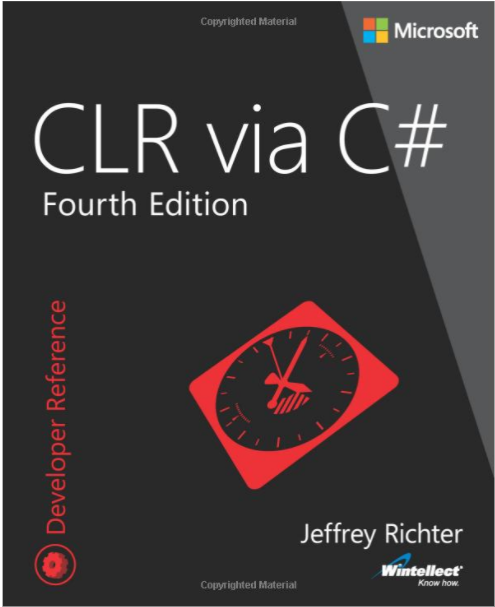
\includegraphics[width=0.6\textwidth]{clrViaCSharpCover.png}
                \end{center}
            \end{column}
        \end{columns}
    \end{frame}

\end{document}
